\documentclass{jot}

\usepackage[utf8]{inputenc}
%\usepackage[T1]{fontenc}
\usepackage[english]{babel}
\usepackage{microtype} % optional, for aesthetics
\usepackage{tabularx} % nice to have
\usepackage{booktabs} % necessary for style
\usepackage{graphicx}
% \graphicspath{{./figures/}}
\usepackage{listings}
% \lstset{...}

% \newcommand\code[1]{\texttt{#1}}
% \let\file\code

%%% Article metadata
\title{Reflections on OCL~2.}
\runningtitle{Reflections on OCL~2}

\author[affiliation=orgname, nowrap] % , photo=FILE]
{Edward D. Willink}
{is the chair of QVT and OCL specification Revision Task Forces at the Object Management Group and project leader for QVTd and OCL at the Eclipse Foundation.
	Contact him at \email{ed \_at\_ willink.me.uk}.}

\affiliation{orgname}{Willink Transformations Ltd., Reading, UK,}

\runningauthor{Edward D. Willink}

\jotdetails{
	volume=V,
	number=N,
	articleno=M,
	year=2011,
	doisuffix=jot.201Y.VV.N.aN,
	license=ccbynd % choose from ccby, ccbynd, ccbyncnd
}

\begin{document}

\begin{abstract}
	
Twenty years after the OCL~2.0 Request For Proposals, it is perhaps long overdue for a review as to how well the resulting semi-formal OCL~2 specification makes the informal OCL~1 specification more precise. We briefly relate the history that allowed an imprecise draft to be adopted by the OMG as the OCL~2.0 specification resulting in a language that was fatally flawed from the outset. We draw on personal experience to explain why recognition of the fatality of the flaws has taken so long. However despite these flaws, OCL remains the language of choice for specifying model constraints. Therefore armed with an understanding of the flaws, we make practical suggestions for how an OCL~3.0 might resolve them.

\end{abstract}

\keywords{OCL, Object Constraint Language, Precise specification, Side effect free}

\section{Introduction}

The UML specification arose to resolve the `method wars' that left users confused as to whether a class should be drawn as a cloud or rectangle. In this respect UML has been a total success, but obviously there is more to modeling than classes, and as soon as models become non-trivial, additional constraints are required that cannot be sensibly expressed graphically. The UML~1.1~\cite{UML-1.1} suite of documents therefore includes a document defining the OCL~1.1~\cite{OCL-1.1} textual language that can elaborate UML diagrams.

The OCL language evolved from work on the Syntropy method at IBM, and in so far as many thousands of academic papers have successfully used OCL to express constraints, OCL too has been a total success.

In Section~\ref{History} we relate the history of the OCL~1 to OCL~2 transition before examining the problems with OCL~2. We firstly examine the language problems directly affecting users in Section~\ref{Language Problems} and then the specification problems that directly affect toolsmiths and indirectly affect users in Section~\ref{Specification Problems}. Then in Section~\ref{OCL Building Block} we consider what a useful OCL Building Block might look like and what an OCL~3 might do to support it. Finally in Section~\ref{Conclusion} we conclude.

\section{OCL~1 to OCL~2 History}\label{History}

The software community was not satisfied to leave UML (and OCL) as a useful flexible semi-formal facility for communicating analysis considerations. Rather a near-formal semantics for UML (and OCL) was required to specify behavior precisely and so facilitate synthesis of functional code direct from UML diagrams. 

The formality of OCL was addressed by Martin Gogolla's student Mark Richters whose PhD thesis~\cite{Richters} was adapted to provide the formal Annex that accompanies all the OCL~2.x specifications. Ir provides a useful reference to help resolve issues in the main specification, however since the Annex has not tracked all the OCL~2 evolutions, sometimes the Annex just contributes to a contradiction for implementers and users to reconcile.

\subsection{OCL~1.5}

Reviewing the final version of the OCL~1 specification embedded within the UML~1.5 specification~\cite{UML-1.5}, we find a nice simple 50 page informal exposition of:
\begin{itemize}
	\item{the language from a user perspective}
	\item{the library operations from a user perspective}
	\item{an EBNF grammar}
\end{itemize}

This could be called a black box specification. It reveals what the user sees. It imposes no limitations on how an implementation satisfies the specification. With so little detail, most of the problems of the 210 page OCL~2.0~\cite{OCL-2.0} do not exist. However some do.

OCL~1 supports open classes in so far as let-operations and let-attributes define new pseudo-operations and pseudo-attributes for the exclusive use of the OCL. No clues about how pseudo-operations and pseudo-attributes are modeled in UML is given.

OCL~1.5 claims that `A parser generated from this grammar has correctly parsed all the constraints in the UML Semantics section, a process which improved the correctness of the specifications for OCL and UML.' This is patently untrue since skipping over obvious formatting typos such as the \verb$Guard$ invariant, many of the constraints have failed to track the language evolution that mandates empty parentheses on parameterless operations and replaces the \verb$#$ syntax for enumerations by qualified names.

UML~1.x has \verb$Attribute$s, \verb$AssociationEnd$s, \verb$Operation$s and \verb$Method$s for which OCL~1 uses the generic term `property'. Unfortunately when UML~2.0 unified the \verb$Attribute$ and \verb$AssociationEnd$ classes as the \verb$Property$ class, the OCL text failed to track uniformly; the resulting OCL~2 text can be rather confusing.

OCL~1.x uses the term `stereotype' to refer to the \verb$inv$/\verb$pre$/\verb$post$ discriminant. This is confusing to any reader who may be familiar with the UML \verb$Stereotype$ class and its capabilities.

OCL~1.x specifies that all collections are always flattened.

OCL~1.x recognises that non-collection values may be `null', but does not provide any clues as to what this may mean semantically.

OCL~1.x does not specify what happens if the index-is-in-range precondition for \verb$Sequence::at$ is not satisfied. OCL~1.x does not specify a no-divide-by-zero precondition on \verb$Real::/$.

OCL~1.x specifies that the Standard Library is a modeled \verb$Package$ and specifies how it may be extended by another \verb$Package$ using an \verb$«OCL_Types»$ dependency. No model for the Standard Library is provided and so the specified extension is not practical. 

\subsection{UML~2.0 submissions}

The two competing UML~2.0 submissions~\cite{UML-2U},\cite{UML-U2P} both recognized the utility of OCL and also recognized that OCL had utility beyond UML. OCL was therefore excluded from the responses to the UML 2.0 RFP~\cite{UML-2.0-RFP} and treated as a new self-standing specification with its own RFP~\cite{OCL-2.0-RFP}. This separation was very convenient for the UML teams and in many respects good for OCL too, but unfortunately the separation from UML and the drive to better formality required many extra problems to be addressed. When the UML teams ran out of enthusiasm / resources, the result was a work in progress draft~\cite{OCL-2.0-draft}.

The draft OCL sat on the shelf at OMG for three years until seven out of eight of the competing QVT specification submissions agreed that the QVT specification should exploit OCL. The QVT specification~\cite{QVT-1.0} could not be adopted until the OCL~2.0 specification had been adopted and so the work in progress draft was dusted off, polished slightly and adopted leading to the official OCL~2.0~\cite{OCL-2.0}. It is unclear how this could have happened since the draft clearly lacked the required prototyping required by OMG, and contains many TBDs to be resolved once UML~2.0 was finalized. UML~2.0~\cite{UML-2.0-adopted} was of course adopted three years prior to this OCL~2.0 adoption. The TBDs persist to this day and are even present in OCL~2.3.1~\cite{OCL-2.3.1} which was adopted as an ISO standard; perhaps the only ISO standard with explicit TBDs and prolific known inconsistencies.

\subsection{OCL~2.0 aspirations}\label{OCL~2.0 aspirations}

Whereas OCL~1.x was a black box specification, OCL~2.x is a white box specification. It specifies the Abstract Syntax (AS) model for OCL with the excellent intention that this should facilitate interchange using XMI between alternative OCL tools. Unfortunately this model was not provided until OCL~2.2~\cite{OCL-2.2} and even then it is not quite right since no prototype had been built.

As an evolution of OCL~1.x, it was natural for the OCL AS model to re-use UML metaclasses. However once the UML-OCL connection was severed, the use of such a bloated and in some respects inadequate foundation should have been reconsidered. The re-use of UML became untenable once OCL~2.0 Section 13 added the claim that EssentialOCL could work with EMOF.

Specification of the AS model required that the conversion between the grammar and the AS be specified as well. This is achieved by specifying a non-normative Concrete Syntax (CS) model that closely resembles the grammar, and a variety of rules mapping grammar to CS and CS to AS. Since the grammar is ambiguous, a further category of disambiguating rules is required. The exposition of this conversion burden is arranged around the non-normative CS classes, for which no model has been provided. This avoids revealing how far from correct the CS classes are. The coherent OCL~1.5 grammar is replaced by CS-relevant snippets scattered throughout the chapter. As a minimum this imposes a major cut and paste burden on any developer attempting to use them. More practically, it obfuscates to such an extent that a casual reader is impressed by the apparent detailed formality and unaware of the total absence of any prototyping to substantiate the unusable content.

Standardization of the AS requires that the internal awkwardness of OCL~1.x's pseudo-attributes and pseudo-operations be properly modeled. They are not and to make matters worse the pseudo-attributes and pseudo-operations are elevated to attributes and operations that can be used just as if they were part of the original model. This is tantamount to providing open classes and presents an unresolved challenge when the AS model is serialized as XMI.

The availability of an AS model provided an opportunity to specify the execution semantics. The exposition is semi-formal and uses a rather obvious and incomplete \verb$ValuesPackage$ and \verb$EvaluationPackage$. %How can if-then-else be specified without presupposing its semantics? \verb$IfExpEval$ avoids the problem by leaving the condition/then/else to result value relationships to the readers intuition.

The \verb$EvaluationPackage$ makes a first attempt at temporal modeling using a \verb$LocalSnapshot$ class to maintain a history of object states. I'm not aware of any implementation that uses this aspect of the specification. The relatively recent work on sequences of system snapshots (filmstrips~\cite{Desai}) by Martin Gogolla's team at Bremen~\cite{USE} seems much more promising.

\subsection{OCL 2 Architecture}

\begin{figure}
	\begin{center}
		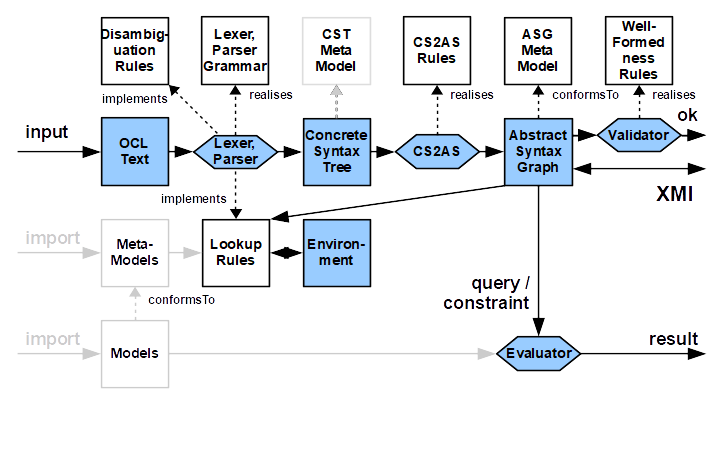
\includegraphics[width=4.5in]{OCL2Architecture.png}
	\end{center}
    \vspace{-40pt}
	\caption{OCL 2 Architecture}
	\label{fig:OCL2Architecture}
\end{figure}

Fig~\ref{fig:OCL2Architecture} shows the components of the architecture implied by the specification. Along the top row, transparent boxes show different aspects of specified behavior that configure the shaded concrete boxes realized by the tooling on the second row. Input text is lexed and parsed to give a Concrete Syntax Tree that is converted to an Abstract Syntax Graph and then validated.

The troublesome ability to interchange the ASG using XMI is indicated.

A non-standard parser is required since it must implement the disambiguation rules and lookup rules. The lookup rules cannot be expressed in pure OCL since they create and modify new \verb$Environment$s for each construct such as a \verb$LetExp$ that introduces a nested scope. The mechanism by which the user-metamodels are imported and the construction of a root \verb$Environment$ is greyed out since it is unspecified.

The bottom row shows how the parsed ASG provides a query or constraint that an evaluator may use to provide a result, using models whose import mechanism is again unspecified.

Before criticising OCL~2 too harshly, it must be remembered that there were no metamodels for OCL~1 and so the metamodels for OCL~2 were a significant novelty. We should perhaps praise the OCL~2 metamodels for being perhaps 95\% correct rather than dwelling on the 5\% wrong. However it is the 5\% wrong and the lack of a comprehensive prototype to reveal the wrongness that has caused so much trouble.

\subsection{Author's Background}

Since parts of this paper rely on the personal observations of one of the leading participants at OMG and Eclipse, it is appropriate to provide a selective biography to distinguish my direct and indirect knowledge.

My involvement started in around 2003 from providing Eclipse support for the UMLX model transformation language~\cite{Willink-UMLX} using the then planned QVTr language. This led to participation in the Eclipse support for QVTr and interaction with the Eclipse OCL project~\cite{Eclipse-OCL} to make it extensible for use by the Eclipse QVTd project~\cite{Eclipse-QVTd}. I had no involvement with OCL~2.0. I contributed a few review comments to QVT 1.0.

Involvement with OCL and QVT at Eclipse led to the my appointment as the Thales representative for the OMG Revision Task Forces for OCL and QVT. I therefore contributed some revisions for OCL~2.2 and consistent models for QVT 1.1.

As personnel at OMG and Eclipse moved on, I found himself as chair of the OMG OCL and QVT RTFs and as project lead of Eclipse OCL and QVTd projects. Lack of active personnel meant that I was often the sole active participant.

I `retired' from Thales in 2012. Since then I am grateful, firstly to Tricia Balfe at Nomos Software, and then to Cory Casanave at Model Driven Solutions, for appointing me as their OCL and QVT RTF representatives.

At OMG, I resolved the `easy' problems in OCL~2.3 and OCL~2.4. This led to increasing awareness of the `hard' problems and the issuing of a Request For Proposal to address these via an `OCL~2.5' rewrite. The RFP~\cite{OCL-2.5-RFP} can be read as a catalog of the serious OCL~2 problems.

At Eclipse, I inherited the Classic Eclipse OCL for Ecore/UML whose stable APIs made significant development almost impossible. A new fully-modeled Eclipse OCL exploited Xtext to provide much enhanced UX and a Pivot model to unify the competing Ecore and UML needs. Enhanced APIs and Java code generation support extension for QVT. The Pivot-based Eclipse OCL prototyped many solutions for OCL specification problems. Many of the solutions have been presented to the annual OCL Workshop. Unfortunately the need for API stability has become a hindrance to further development.

\section{Language Problems}\label{Language Problems}

Problems with the OCL language have a very direct impact on the user and may require users to program in an unnatural style to circumvent the limitations.  

\subsection{Program Failure}

An inevitable characteristic of any manually developed program is that it may malfunction and consequently the program language and execution support must accommodate failures. Failures typically take one of two forms.

\paragraph{catastrophic failure} A catastrophic failure is often called a crash. It may occur from a hardware, software, network, or I/O system failure. Programs cannot normally recover from these failures and so the execution launcher will normally attempt to provide as much helpful diagnosis of the failure as possible before terminating execution abruptly.

\paragraph{recoverable failure} A recoverable failure may occur when the programmer finds it convenient to reuse some failure detection code and then to compensate for the failure, typically by catching a thrown exception.

%exploit failure detection within some invoked module than to duplicate the detections and so avoid the failure. A simple example of this occurs when a Java \verb$NumberFormatException$ is caught after using \verb$Double.parseDouble$ to convert a string representation of a number to a number. In this case programming a syntax check would be a waste of effort and execution time.

\paragraph{not-a-failure} Conversely a programmer may correctly anticipate a failure and provide a guard to direct the program control to bypass and so avoid the failure. 

In Java the two actual failure cases are separated by using \verb$Error$ or \verb$RuntimeException$ for catastrophic failures and by using \verb$Exception$ for recoverable failures. \verb$Exception$s form part of a Java function signature and so there can be some static diagnosis of code that neglects to handle the recoverable failures.

OCL~1 has preconditions but provides no indication of how an evaluation should behave when a precondition is not satisfied. OCL~2 is similarly vague and so OCL~2 tools often treat the corresponding preconditions (and postconditions) as just syntax-checked comments to document a hazard for a human reader.

OCL~2 pursues a functional approach and, in the event of a malfunction, returns a regular \verb$invalid$ value rather than imposing an alternative `return' mechanism for an \verb$Exception$. The \verb$invalid$ value can be `caught' by using the \verb$oclIsInvalid()$ library function. This is different to many languages but more regular and so perhaps better.

Unfortunately the OCL~2 specification is not really concerned with failures for which it mandates that \verb$invalid$ is a singleton; all failures are the same and free from any helpful diagnostic detail. Some OCL tools ignore this stupid restriction and provide a rich \verb$invalid$ that propagates diagnostics while preserving OCL semantics by ensuring that the diverse \verb$invalid$s behave as one.

The lack of consideration for crashes forces an OCL~2 implementer to use the \verb$invalid$ return for all crashes.% and to ensure that they can be caught be \verb$oclInInvalid()$.

The OCL specification provides no ability for the use of \verb$invalid$ to be declared as part of a function signature, consequently OCL, whose strong side effect free formality supports strong analysis, has a gaping hole in regard to guaranteeing that a program execution will not fail.

\subsection{2-valued Booleans and invalid}

Almost every gathering of the OCL community provokes discussion of why OCL Booleans are not 2-valued \{\verb$true$, \verb$false$\}. Clearly many OCL users are unhappy with the prevailing 3-valued \{\verb$true$, \verb$false$, \verb$invalid$\} specification \footnote{The idempotent addition of a null as a fourth output in OCL~2.4 is a further but irrelevant confusion.}.

But this is all a misunderstanding. In OCL, as in other languages, a non-trivial Boolean-valued calculation has three possible outcomes; success/\verb$true$, failure/\verb$false$ and crash/\verb$invalid$. When the crash is realized as a thrown exception, the programmer can ignore the crash outcome and code as if there were only two possible outcomes. Exactly the same programming approach is possible with OCL provided the programmer ensures that the particular OCL tooling API such as \verb$check()$ that is used for the evaluation is `strict'; i.e. it converts the \verb$invalid$ or \verb$null$ value returned by OCL to a crash by throwing an exception. The OCL tooling may offer an alternative API such as \verb$evaluate()$ that returns all three outcomes as OCL values. This alternative is useful when the programmer really wants to program all three outcomes, but is the probable source of unhappiness when only two outcomes were expected.

\subsection{Short-circuit operators}

In many C-based programming languages short-circuit and/or operators support a guard idiom to ensure that ensures that the evaluation of a first term converts the crash that would result from evaluating the second term to not-a-failure.

\begin{verbatim}
    (x != null) && x.doSomething()
    (x == null) || x.doSomething()
\end{verbatim}

OCL appears to be much the same:

\begin{verbatim}
    (x <> null) and x.doSomething()
    (x = null) or x.doSomething()
\end{verbatim}

but since the operators are commutative the following must return the same results 

\begin{verbatim}
    x.doSomething() and (x <> null) 
    x.doSomething() or (x = null) 
\end{verbatim}

An optimizing implementation or a multi-processor implementation may evaluate the two terms in arbitrary order. An implementation may be unable to avoid the crash, so it must instead catch the crash from the `wrong' term and suppress it once the guard from the `right' term is determined. The not-a-failure is not necessarily avoided.

This is not what was intended when the Amsterdam Manifesto~\cite{OCL-Amsterdam} adopted the Kleene logic to support short-circuit rather than `strict' Boolean operators. The extended Truth Table for the \verb$and$ operation was and is.

\begin{center}
	\begin{tabular}{|c||c|c||c|}
		\hline
		Use Case & Input 1 & Input 2 & Output \\
		\hline
		\hline
		2-valued & false & false & false \\
		& false & true & false \\
		&  true & false & false \\
		& true & true & true \\
		\hline
		Normal Short-Circuit & false & X & false \\
		Commutated Short-Circuit & X & false & false \\
		\hline
		Residue & true & X & X \\
		& X & true & X \\
		& X & X & X \\
		\hline
	\end{tabular}
\end{center}

The table has been redrawn here to distinguish the four 2-valued Boolean cases, the two short-circuit cases and three residual cases.

In the Amsterdam Manifesto, `X' was spelled as `undefined' and was clearly described as a virtual value meaning not-yet-computed in order to explain how the two short-circuit cases yield a useful result without needing to compute a redundant and quite possibly uncomputable term.

In OCL~2.0 and 2.2, `X' is spelled as `$\bot$' to represent a \verb$null$ or \verb$invalid$ value. Whether the output is \verb$null$ or \verb$invalid$ was unclear.

In OCL~2.3, `X' is spelled as `$\epsilon$' or `$\bot$' respectively for a \verb$null$ or \verb$invalid$ Input value and explicitly just \verb$invalid$ as an Output.

In OCL~2.4, `X' is again spelled as `$\epsilon$' or `$\bot$' for an Input value but as an idempotent `$\epsilon$' or `$\bot$' as an Output.

The 2-valued cases are uncontroversial.

The Short-Circuit cases solve the problem of choosing a Truth Table row when one of the input values cannot be computed since the short-circuit rows are available for use by not-yet-computed inputs. There is no need to attempt to compute what cannot be computed.

%The Commutated Short-Circuit row is the inevitable consequence of a commutative \verb$and$ operator. While this may be mathematically elegant, it makes for a stupid implementation, since an implementation that optimises or uses multiple processors may easily compute the `wrong' argument first. This mandates that the implementation `catch' the consequence of malfunction of the `wrong' argument and ignore it once the `right' argument yields a \verb$false$ guard. In so far as OCL evaluation is side effect free, the only observable side effect is a waste of CPU time, but any user of a debugging or tracing tool will be confused by the chaos that may arise during the redundant failing evaluation of the `wrong' argument. While there is nothing mathematically wrong with the Commutated Short-Circuit, there is nothing practically useful and many things are practically damaging. It may also surprise users, used to traditional short circuit operators, if a crash while evaluating the first term is `rescued' by a \verb$false$ second term.

In so far as the Residual Use Cases describe the propagation of the virtual not-yet-computed value there is nothing wrong with them. However program execution does not normally reify the not-yet-computed result; rather we twiddle our thumbs waiting for the computation to complete or fail.

The virtual not-yet-computed meaning of `undefined' in the Amsterdam Manifesto evolved to the actual values of \verb$invalid$ and \verb$null$ in OCL~2 so that the Residual Use Cases no longer describe not-computations but failure propagation. %For OCL~2.0 and 2.2, as clarified in OCL~2.3, the residual use cases all result in \verb$invalid$ giving the desirable alternatives of a 2-valued or crash evaluation. The only problem would appear to be that whereas in Java, an \verb$Exception$ will propagate through the calling logic by default, for OCL-based evaluation the calling logic must be `strict' to ensure the same \verb$invalid$ propagation and so avoid the need to handle more than the \verb$true$ or \verb$false$ alternatives.

%For OCL~2.4, I was persuaded by the team formalizing OCL using Isabelle that the OCL~2.3 clarification of 4-valued input, 3-valued output Boolean logic was not idempotent. The changed 4-valued output for OCL~2.4, may be more elegant mathematically but it is certainly no better practically. How can anyone justify that

%\begin{verbatim}
%    null and null
%\end{verbatim}

%is anything other than a bad Boolean evaluation? It must be \verb$invalid$, a full failure, not \verb$null$, some kind of lesser failure. I very much regret making this change and apologize. I should have made clear that OCL~2.3 Boolean operations are really 3-valued input, 3-valued output with a `strict' preprocessor that, just like Integer or String operations, treats each \verb$null$ input as \verb$invalid$.

%While the above considerations identify some strange characteristics of the OCL Boolean operators, there is nothing actually wrong, so why are users unhappy. In Java a non-trivial Boolean calculation has three outcomes \{\verb$true$, \verb$false$, \verb$crash$\} and in OCL we also have three outcomes \{\verb$true$, \verb$false$, \verb$invalid$\}. The problem must therefore be a misunderstanding. In Java the \verb$crash$ propagates and so the Java programmer can ignore it and program as if there were only the two outcomes \{\verb$true$, \verb$false$\}. The same Java programmer handling the return from an OCL-in-Java may find that e.g. the \verb$evaluateConstraint$ API returns a distinct value for each outcome, requiring the programmer to program strictness explicitly by converting the OCL \verb$invalid$ or \verb$null$ value to a Java \verb$Exception$. If the programmer does not understand about strictness, unhappiness may result. Alternatively there may be an alternative e.g. \verb$checkConstraint$ API that provides a two-valued Java result after performing the strictness check as part of its operation; the Java programmer may now be happy.

%In conclusion, much of the unhappiness may be due to poor OCL-in-Java APIs provided by OCL tools, and misunderstanding of the need for strictness by Java programmers.

Similarly the commutative and short-circuit characteristics of the Boolean operators, when implemented, conflict with the not-a-failure intent of the Amsterdam Manifesto. This causes surprise to the user of a debugging or tracing tool who may observe the chaos of a failing redundant computation, and a further surprise to a user who finds that a crashing first term is rescued by a second term. This potential of the commutated short-circuit for surprise, inefficiency and implementation difficulty may justify a change to a traditional non-commutative short-circuit. It is not clear that the mathematically elegance of commutative and/or provide any practical benefits; they certainly provide considerable implementation difficulties.

%I remain puzzled that the desirable mathematical properties of commutativity and idempotency have conflicted with practicality for OCL.





%Thus \verb$false and undefined$ can be evaluated as \verb$false$ without actually computing the second argument. As a virtual value, `undefined' would be better phrased as `not yet computed'.

%The virtual value appears to solve the problems; guarding works and even appears to be `strict' in so far as all computed \verb$null$ or \verb$invalid$ values can propagate as \verb$invalid$.

%Unfortunately the Kleene logic also specifies that \verb$and$ is commutative and so \verb$undefined and false$ must also evaluate to \verb$false$. Typical implementations will evaluate the first term as \verb$invalid$ before discovering that the second term is \verb$false$. The implementation must therefore violate strictness by caching the \verb$invalid$ while the second term is evaluated allowing the \verb$undefined and false$ Truth Table entry to be used to determine the value of \verb$invalid and false$.

%The same problem can arise with the forward guard, since commutativity allows an implementation to optimize execution to evaluate arguments in either order or even concurrently.

%The need to reify the `not yet computed' virtual value and the inappropriate correlation of the actual \verb$invalid$ and \verb$null$ values with the virtual value explains many confusions in the OCL specification. 

%\subsubsection{Short-Circuit Boolean evaluation}

%Clearly commutativity is incompatible with the guard idiom and the implementation of \verb$undefined$ as a virtual value that is never reified.

%If we reject commutativity and instead use the short circuit semantics that programmers have found very satisfactory in C and its successors, the problems vanish; any actual use of \verb$null$ or \verb$invalid$ in a Boolean operation is evaluated as \verb$invalid$. The short circuit functionality allows the first argument to inhibit the unwanted computation of a \verb$null$ or \verb$invalid$ second argument.

%The functionality is `strict', however the \verb$and$, \verb$implies$, \verb$or$ operations just like \verb$if then else endif$ have sequenced and selective argument evaluation.

%\subsubsection{Guard Syntax}

%Either the guard idiom or commutativity must go, so if commutativity is paramount, a %distinct syntax must be introduced 

%\begin{verbatim}
%    (x <> null) guards x.doSomething()
%\end{verbatim}

%This would be an OCL novelty almost deliberately conflicting with a widespread practice. A new clearer explicit syntax seems a poor trade off for user confusion.

%and to determine the answer we must lookup the left and right hand value in a Truth Table. For the case where x is \verb$null$ we look up {false and invalid} to compute false. Since and is commutative there is no difference in writing

%\begin{verbatim}
%x.doSomething() and (x <> null)
%\end{verbatim}

%and entering the Truth Table at {invalid, false} to compute false.

%This is consistent with commutativity but very surprising since most languages offer asymmetric short circuit boolean operations. It is also inconvenient for practical tooling since both arguments are of equal importance and so should be evaluated prior to Truth Table lookup.

%The design decision to break strictness to support a Kleene Boolean algebra seems to offer no benefits to the user or a practical implementation. Rather it has irritated nearly everyone.

%Eclipse OCL has finally added alternative and2, implies2, not2, or2, xor2 operations that exhibit conventional strict, short-circuit 2-valued behavior. Execution and code generation is considerably enhanced.

%\subsection{2-valued Booleans and null}

%UML defines a [?] multiplicity for values that may be null in support of the very common idiom that a slot is set by a constructor to a null value and subsequently assigned a non-null value once an appropriate initialization has completed. OCL, like Java, supports this via a null value.

%A problem arises when null values appear as inputs of Boolean operations.

%With a strict interpretation, null is bad so the result is simple; null values crash. But with commutative Kleene functionality null and null gives a null result. At best this can be confusing. There are six possible logics for {true, false, null} depending on which of the alternatives is more `important' than another. I attempted to use OCL's Boolean for a 3-valued  state, but my required logic priority differed from OCL's. It would appear that since OCL's Boolean operations for null can only be suitable for one user in six,the facility should be retracted to avoid deceiving the five out of six.

%\subsubsection{Rationalization}

%How did this mess arise?

%\verb$null$ is a genuine state of a \verb$[?]$ multiplicity variable that has not been initialized with a more explicit value or which has been explicitly assigned a \verb$null$ value. The concept was inverted by Tony Hoare, endorsed by UML~1 as the value of a \verb$[0]$ multiplicity. It was reified by UML~2 using the \verb$LiteralNull$ class and as a value by OCL~2 as the \verb$null$ literal. OCL~1 did not have a \verb$null$.

%\verb$invalid$ is a genuine value that is returned when an operation such as \verb$Sequence::at()$ has malfunctioned. It was introduced as a value by OCL~2.

%`undefined' is a virtual value used to populate the Truth Table for Boolean operations where the relevant value does not need to be defined. The sleight of hand was introduced by the Amsterdam Minifesto.

%The Formal Annex for OCL defines the special value $\bot$ as the undefined value which is part of the domain of each type, and then elaborates its usage to represent the undefined (null) value or the erroneous (invalid) return. This set the disastrous precedent for treating `undefined' as the genuine \verb$null$ or \verb$invalid$ values rather than a virtual value.

%OCL~2.0 introduced the \verb$oclIsUndefined()$ operation to test whether a value is \verb$null$ and the \verb$oclIsInvalid()$ operation to test whether a value is \verb$invalid$. \verb$oclIsInvalid()$ is not a problem, it provides a mechanism to `catch' the invalid. \verb$oclIsUndefined()$ compounds the disaster. Quite apart from being redundant, \verb$= null$ is shorter and more conventional, it re-inforces the incorrect association of the word `undefined' and the value \verb$null$. Successive maintainers of the OCL specification, including myself, have sought to use only the genuine values \verb$null$ and \verb$invalid$ and rewritten text and the Truth Tables accordingly.

%As a consequence, evaluation of \verb$null and true$ uses the \verb$undefined and true$ entry and returns \verb$null$. If however `undefined' is only a virtual value, there is no Truth Table entry to support \verb$null and true$. This is a pre-condition failure and the result is therefore \verb$invalid$ giving us the strict semantics that we require.

\subsection{Dot and Arrow Navigation operators}

Newcomers to OCL are confused by the difference between dot and arrow navigation operators. Prior to OCL~2.4, the specification was unhelpful and so newcomers fail to discover the simple rule that dot is for objects and arrow for collections. The availability of the implicit-collect and implicit-as-set shortforms give the dot and arrow operators a utility for the `wrong' sources. This can confuse even experienced OCL programmers.

\begin{verbatim}
    myCollection->collect(name)      -- explicit collect
    myAggregate.name                 -- ?? implicit collect ??
\end{verbatim}

The utility of implicit-collect is mixed. Some users like the compact exposition of some constraints. Other users dislike the ease with which a typo acquires an unexpected meaning. In the second example above, the use of a singular word such as \verb$myAggregate$ makes it impossible to tell locally whether \verb$name$ is a property access of the \verb$myAggregate$ instance of a \verb$MyAggregate$ class, or an implicit collect of the elements of a \verb$myAggregate$ collection.

Prior to OCL~2.4, the implicit-as-set was ill-specified and not a shortform. The introduction of the explicit \verb$oclAsSet$ library operation formalized the shortform.

The EOL variant of OCL used by the Epsilon~\cite{Eclipse-Epsilon} transformation languages demonstrates that it is possible to make do with just a dot operator for both objects and navigations. The user confusions are eliminated.

A clearer OCL could similarly use just a dot operator. The brevity of implicit-collect could be rescued by defining a \verb$*.$ navigation operator which reads naturally as many-dot for an implicit-collect shortform.

\begin{verbatim}
    myAggregate*.name                 -- shortform explicit collect
\end{verbatim}

A similar \verb$.*$ shortform which reads as dot-to-many could rescue the implicit-as-set, but this usage is probably too rare to merit the shortform.

%\subsection{Precision}
%UML misdirection
%Model
%-- URI

%\subsection{Library}\label{Library}
%Utility
%Types
%Extensibility

\subsection{Implicit Source}

\paragraph{implicit-self} OCL, like many Object Oriented languages, allows the \verb$self$ start point of a navigation to be omitted. Since the \verb$self$ context is so important, this is very reasonable and can improve readability.

\begin{verbatim}
    name                 -- self.name
\end{verbatim}

\paragraph{implicit-source} OCL, unlike other languages, has powerful collection iteration capabilities and allows the start point of a navigation from an iterator to be omitted.

\begin{verbatim}
    aCollection->isUnique(name)   -- aCollection->isUnique(e | e.name)
\end{verbatim}

This again may aid readability by shortening the exposition. Unfortunately it also adds confusion since the tool and a reader must decide which of many possible implicit-sources in a nest of multi-iterator iterations or an implicit-self has been omitted. Typos and misunderstandings are too easy.

Within iterator bodies, only the first iterator of the most nested iteration should be available as an implicit source, self should be explicit.

\subsection{Reflection and oclType()}

Reflection is little used in OCL, perhaps because the OCL~2 specification has repeatedly changed the semantics of \verb$oclType()$ seemingly in an effort to find a valid way of providing access to the name of a type without imposing the baggage of a fully reflective type system.

The reflective OCL~1 seems much clearer and supports the usage within some of the OCL~2 constraints.

\subsection{Precision}

As a specification language, OCL specifies unbounded precision for its ideal Integer and Real calculations. This is clearly unrealistic and inefficient for many practical applications where 16 bits is often enough for counters and sequence indexes.

In practice, the type declarations of the model slots from which values are read provides a strong clue as to what precision is appropriate, but it is only a clue. To avoid implementation guesswork, there should be a mechanism for OCL evaluations to specify precision, overflow and underflow behavior.

\subsection{Libraries}

One of the most impressive characteristics of Java is how its Object polymorphism enabled it to launch with powerful Collection libraries that have grown and grown. C++ lagged horribly. OCL still lacks support for standard or user libraries the most obvious of which would be a maths library.

\section{Specification Problems}\label{Specification Problems}

Problems with the specification are mostly a concern for toolsmiths, since they must work hard to find workarounds for the difficulties. The problems are only apparent to users when the workarounds lead to disappointing or confusing functionality or incompatibility between alternative tools. Sadly the two best OCL implementations, USE and Eclipse OCL, are seriously incompatible and address very different use cases. 

\subsection{OCL~1.1 Grammar}

Prior to the availability of LALR support tools such as yacc~\cite{YACC}, it was understandable that language specifications might be imperfect; thus C suffers from the notorious dangling-else ambiguity which all C/Java programmers learn about the hard way.

With the availability of yacc, it is inexcusable for any language to fail to provide a yacc grammar. The OCL~1.1 grammar dates from 1997 (22 years post-yacc). It is an EBNF grammar that can be converted to LALR form without too much trouble. Converting to LALR form reveals a multiplicity bug, a name conflict and lexer comments that are easily resolved. It also reveals a very serious shift/reduce conflict when parsing a property call such as \verb$x.y(z1, z2, z3)$. A potentially large lookahead is needed to search for the \verb$|$ that distinguishes the iteration call \verb$y(z1, z2 | z3)$ from the operation call \verb$y(z1, z2, z3)$. 

The OCL~1.1 grammar is bad; it is incompatible with standard tooling. If LALR tooling had been used, the OCL syntax would have been adjusted.

The free parser advertised by the specification is no longer available from the IBM website making it impossible to determine how the ambiguity was resolved.

\subsection{OCL~2.1 Grammar}

At least the OCL~1.1 grammar exists as a nearly coherent whole; it can be cleaned up from a cut and paste from the specification PDF. For OCL~2.0, which is only a draft, the grammar was split up and interleaved with inherited and synthesized attribute rules. Distinct rules `clarify' each different form of navigation. This introduces many ambiguities necessitating some disambiguation rules. These difficulties are aggravated by partial name refactorings corresponding to work in progress tracking UML~1 to 2 evolution. Further difficulties arise from incomplete evolution to accommodate qualified names and static operations.

Eventually I have come to accept that the OCL~2.x grammar and CS rule specifications are not fit for purpose. Each implementer is obliged to empathize with the spirit of the specification and code accordingly. It is not surprising that few tools fully support the complexities of unnavigable opposite navigation or association classes.

I developed a yaccable version of the OCL~2 grammar for inclusion in the OCL~2.3 revision, but retracted it at the last moment when it became clear that the left recursion typical of LALR tools was troublesome for the LL tools such as Xtext~\cite{Eclipse-Xtext}. 

\subsection{Other Problems}

There are too many other problems to address here. Some are listed in the `OCL 2.5' RFP~\cite{OCL-2.0-RFP} and others as part of the revisions in Section~\ref{Specification Revisions}.

\section{OCL Building Block}\label{OCL Building Block}

The liberation of OCL from UML was intended to make OCL more generally useful. It is therefore particularly irritating when a user asks `how can I re-use OCL in my application'? This is irritating because the honest answer is that you can't unless you devote considerable skilled programming effort. Why is it so hard?

\subsection{OCL Re-Use Cases}

We first examine a couple of use cases that OCL could respond to and then look at how OCL could make them much easier. This leads us on to some ideas for OCL~3.

\subsubsection{Novel OCL}

If the user has a novel application such as using OCL as a replacement for XPath in the XML/XSD technology space, there are two obvious choices.

\paragraph{Re-implement} A custom implementation can obviously satisfy all the user's requirements, but it requires the user to become familiar with all the complexities of OCL and to rediscover solutions to the many inadequacies of the OCL specification.

\paragraph{Re-Use} Re-use of existing functionality is often preferable, particularly if a re-usable implementation is available. Unfortunately the lack of a clear architecture in the specification encourages the proprietary struggles for solutions to pervade the implementation. It is not re-usable.

Wilke~\cite{Wilke-Variability} highlighted the lack of architecture nicely by identifying that an OCL implementer had two significant design choices to accommodate the user's preferred metamodel representation (UML, Ecore, XSD, Java, ...) and a further two design choices for the user's preferred model representation (Ecore, XML, Java, ...).

\paragraph{Denormalized metamodels} If the OCL functionality is to specify expressions for a particular metamodel representation, the OCL tooling can be coded specifically for that representation. In practice this means substantial re-tooling for each new metamodel representation. When the Classic Eclipse OCL support for Ecore was enhanced to support UML as well, an attempt was made to mitigate the costs of this re-tooling by introducing long (ten) template parameter lists and a reflective class to polymorphize the non-polymorphic Ecore/UML classes. This led to unpleasant code for all representations and probably made the prospect of supporting a third representation even more daunting.

\paragraph{Normalized metamodels} Alternatively, the OCL functionality can be defined for a normalized metamodel representation. There is then no need to re-tool for another metamodel representation since the OCL tooling using the normalised metamodel is unaffected. It is just necessary to convert the user's new representation to the normalized representation. Dresden OCL~\cite{Dresden-OCL} coined the term Pivot model and realized it by a family of adapter classes. The Pivot-based Eclipse OCL performs a full model transformation from Ecore or UML to Pivot taking advantage of the transformation stage to normalize bloated irregular UML concepts such as \verb$Stereotype$s and \verb$AssociationClass$es.

The cost of providing a new normalization for a new metamodel representation is much less than the cost of re-tooling to denormalize OCL. Since there are comparatively few metamodel objects in an application, the extra memory cost of dual metamodel objects is acceptable.

\paragraph{Denormalized models} When evaluating OCL expressions, it is necessary to access the user models which naturally exist in a denormalized form. This could require re-tooling the evaluator to use the denormalized representation. 

\paragraph{Normalized models} Alternatively each user object could be translated to a normalized form for use by a normalized evaluator.

For the potentially very large numbers of user objects, creating a normalized version of each is unattractive since it is liable to double memory consumption. Conversely re-tooling to denormalize all the OCL library routines that support Boolean, Integer, Real and String calculations is also unattractive. A halfway house is much more practical; use the normalized representation for all the built-in values and the denormalized representation for the user objects. It is then only necessary to perform normalizing conversions as part of the property call evaluation facility that fetches a value from the slot of a user object.

From these considerations we can see that a user with a novel metamodel and model representation could hope to get away with coding
\begin{itemize}
	\item a custom metamodel to normalized pivot metamodel transformation
	\item custom model property access conversions
\end{itemize}

\subsubsection{Bigger OCL}

Alternatively a user may be interested in using OCL as part of a bigger system such as a model transformation language. This is the use case that caused QVT to rescue the OCL~2 draft from oblivion.

It is desirable that the bigger system can re-use as much of the basic OCL as possible and one would certainly hope that the basic evaluation functionality would be reusable; only minor extension should be needed for additional library routines. Extension is self-evidently easier if the specification provides  neutral extensible machine readable expositions such as grammars, metamodels and rules rather than pseudo-code or code. Tool quality is also much improved since code that is auto-generated from grammars, metamodels and rules shares the debugging efforts of other auto-generators. Residual auto-generation bugs tend to have really obvious catastrophic effects. 

%However the technology for grammar tools is not amenable to extension of already compiled functionality, rather the source grammar can be extended and the tooling regenerated.

\subsubsection{Summary}

No matter whether extension occurs for source or compiled functionality, it is very desirable that OCL maximises its ability to be-re-used by providing genuinely re-usable grammars, models and rules. This is the approach that has been pursued by the Pivot-based Eclipse OCL with extension for QVTc or QVTr. However the poor quality of the OCL and QVT specifications have made the extension rather hard.

If OCL is to be easy to extend, it must have a clear specification with a clear architecture. Once these are clear there are opportunities for an implementation to exploit this clarity to produce a correspondingly clear tooling implementation. The clear implementation facilitates selective `borrowing' by a user who really wants to rewrite, and selective overriding by a user who is interested in re-use.

Unfortunately the significant omissions from the OCL specification result in the rather vague architecture shown in Fig~\ref{fig:OCL2Architecture} that practical implementations may ignore completely or revise in proprietary fashion. The net result is poor quality incompatible tools that discourage re-use.



%If a user's requirement is to use OCL as-is then they just need to program their application and exploit the OCL tool support APIs. The user code will be responsible for providing models.

%More likely, the user wants a bigger language of which OCL just forms a part. Model Transformation Languages are examples of this. This lends itself to two alternate architectures.

%The OCL support could be a re-useable component with a limited amount of parameterization with the application independently coded and struggling with the limited parameterzations and APIs. This is the approach offered by the Classic Eclipse OCL and used by Eclipse QVTo and Eclipse Acceleo.

%Alternatively the larger application uses similar technology to the OCL tooling so that each OCL aspect is extended allowing the larger application to be generated as a coherent whole. This is the approach taken by the Pivot Eclipse OCL and used by Eclipse QVTd to support QVTc and QVTr.

%If OCL is to be useful building block it must easily re-useable.

\subsection{Specification Revisions}\label{Specification Revisions}

Once we accept the need to make OCL much simpler and much more re-usable, what should be changed? The main complexity comes from the two distinct CST and ASG metamodels aggravated by the poorly designed grammar that mandates non-standard tooling to support the disambiguation with untimely semantic insights. The grammar can be improved to solve the aggravations, but two metamodels seem unavoidable since the CST is similar to the grammar to ease parsing. The ASG is a compact and sensible information model to facilitate efficient use for execution and analysis.

Exactly the same problems occur in the QVT specifications and so I sponsored Adolfo Sanchez-Barbudo Herrera's EngD~\cite{Sanchez} to provide automated tooling to assist in the awkward CS2AS conversion. This work started in 2013 and so at that time we still lacked the confidence or insight to call out the OCL~2 specification approach as fundamentally unsound.

Let's challenge the presumption that two metamodels are necessary. Figure~\ref{fig:OCL3Architecture} shows a simpler and more regular architecture that might be adopted for OCL~3. We will contrast it with Figure~\ref{fig:OCL2Architecture} to indicate how problems vanish.

\begin{figure}
	\begin{center}
		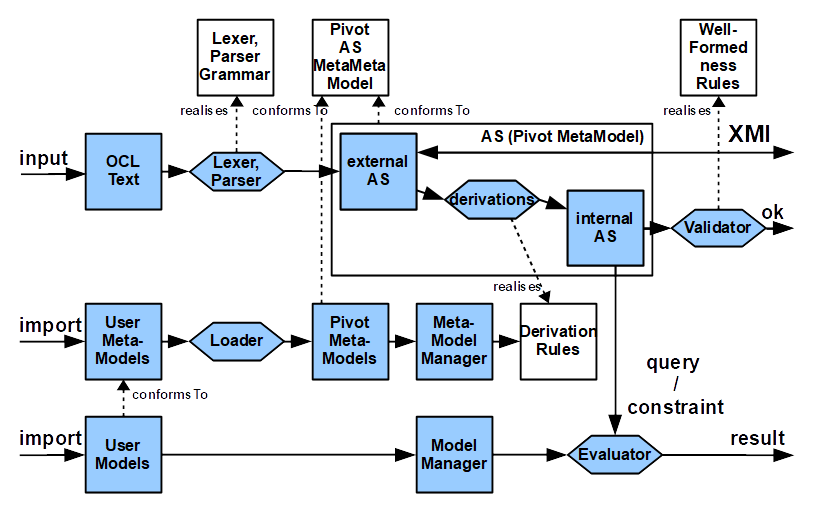
\includegraphics[width=4.5in]{OCL3Architecture.png}
	\end{center}
	\caption{Possible simplified OCL 3 Architecture}
	\label{fig:OCL3Architecture}
\end{figure}

\subsection{Potential OCL~3 Architecture}

The most glaringly missing, greyed out, part of the OCL 2 architecture is the support for user and built-in metamodels (and models). The missing import mechanism, root \verb$Environment$ and treatment of specialized constructs such as \verb$Stereotype$ must be resolved.

\subsubsection{Metamodel Representation}

%OCL~1.x was part of UML~1.x and of course used many UML~1 classes. However OCL~1.x had no metamodel and so it was all a little vague. If OCL~2.x had remained a part of UML~2.x, use of UML~2's bloated and unhelpful classes would be a necessary evil.

%But OCL~2.x was liberated and is free to work with your favourite metamodel representation. Unfortunately the specification requires your representation to be isomorphic to UML~1.x with some UML~2.x tweaks. It certainly cannot be EMOF (or Ecore) or XSD or ... .

\begin{figure}
	\begin{center}
		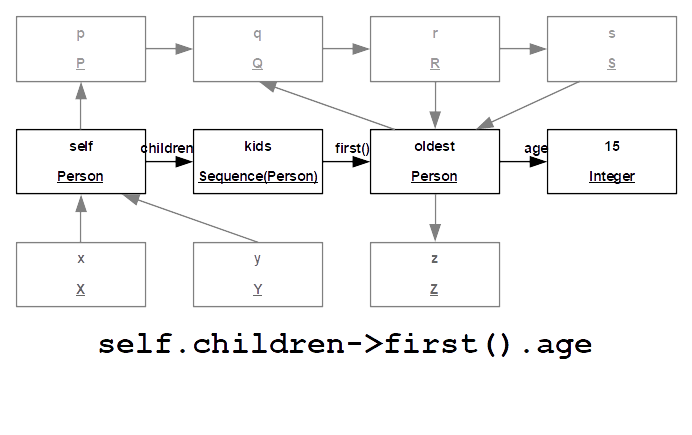
\includegraphics[width=4.5in]{OCLNavigation.png}
	\end{center}
	\vspace{-40pt}
	\caption{OCL Navigation}
	\label{fig:OCLNavigation}
\end{figure}

The enduring success of OCL despite is limitations is probably due to its fundamental simplicity. The state of a system is defined by its many constituent state objects some of whose slots have simple datatype values, while other slots interconnect the objects to form a mesh. OCL evaluation just involves starting at some object, typically known as \verb$self$, and then taking navigation steps from object to object.

Figure~\ref{fig:OCLNavigation} shows a system comprising some arbitrary instances \verb$p$ with correspondingly arbitrary types \verb$P$. In the center row, four objects of interest to an example expression are given more meaningful names and types to show how the example expression steps from object to object in a regular way even though the expression involves collection, operation and datatype complexities.

The figure is clearly a graph in which the nodes can be modeled as instances of classes or as values of specialized classes often called datatypes. These concepts are adequately supported by a variety of metamodel representations.

Edges are more troublesome, since an edge is meaningless without two nodes to define its ends. A minimal modeling of a bidirectional edge that links two nodes identifies the pair of ends. EMOF and Ecore do exactly this with their \verb$Property$ and \verb$EReference$ classes. Unfortunately UML, on which OCL~2 is based, is much more complicated. The edge is modeled by an \verb$Association$ with the ends modeled by \verb$AssociationEnd$s in UML~1 or \verb$Property$s in UML~2. UML adds the even more powerful confusion of an \verb$AssociationClass$ to treat the edge as a node. The UML complexity is clearly excessive for a simple regular OCL treatment.

A further complexity arises with unidirectional edges for which, given a known starting instance, it is only necessary to identify the far edge. EMOF and Ecore may therefore have a property contained by the source instance and referencing the remote instance. Remote navigation is almost impossible. UML also supports unidirectional edges, but changes the containment of the unnavigable end to the association.

As a specification language, it is important for OCL expressions to be able to navigate in both directions~\cite{Willink-Opposites}. But this was not possible using EMOF (or Ecore) until I caused a \verb$Tag$ (or \verb$EAnnotation$) solution to be adopted.

The diverse UML, EMOF or Ecore modeling of edges are all clumsy and a poor basis for a friendly OCL representation. The irregularities are easily normalized away during a transformation to the normalized Pivot metamodel which always has a pair of \verb$Property$ instances to define a bidirectional link between \verb$Class$es and a single \verb$Property$ instance to define the unidirectional link from a \verb$Class$ to a \verb$DataType$ value.

%The state objects are easily modelled as \verb$Class$ instances with \verb$DataType$-valued \verb$Property$ slots. The link between objects can be minimally modeled by a \verb$Property$ at each end of the link. The link `end' class is adequately modeled by a \verb$Property$ in EMOF or \verb$EReference$ in Ecore. UML however models the link as well and so imposes a nearly redundant \verb$Association$ class with \verb$AssociationEnd$s in UML~1 or \verb$Property$s in UML~2 for the ends. For OCL, modeling the link is completely unnecessary; there is no need for a navigation step to stop halfway for a look around. When there really is such a need, UML has the more powerful confusion of an \verb$AssociationClass$ which adds additional unnecessary complexity to the OCL specification. Once adherence to the UML specification is abandoned, \verb$AssociationClass$es can be normalized as regular OCL classes with regular OCL properties for all their possible accesses. \verb$Association$s can be eliminated except perhaps for a lazy reification as a regular OCL \verb$Class$ for backward compatibility with some wacky OCL that really does stop halfway along a link.

%The foregoing dismissal of \verb$Association$ neglects one important complexity; the support for unnavigable opposites. In OCL~2, all links are navigable in both directions regardless of any selective naming or visibility in the user's metamodel. In UML~2, navigable ends are modeled as \verb$Property$ contained by a \verb$Class$, but the \verb$Property$ for an unnavigable end is contained by the \verb$Association$. Unnavigable ends could not be represented in EMOF (or Ecore) until I caused a \verb$Tag$ (or \verb$EAnnotation$) solution to be adopted. These diverse solutions are clumsy and easily normalized away during a transformation to the normalized Pivot metamodel.

Another source of UML complexity arises from \verb$Stereotype$s. These are completely ignored by the OCL specification. The UML~2 specification provides only a minute example from which to extrapolate the, perhaps only possible, coherent design. \verb$Stereotype$s are readily normalized to \verb$Class$es and \verb$Property$s to facilitate regular OCL navigation.

%In summary, the core of the OCL Pivot metamodel needs just well-defined \verb$Class$ and \verb$Property$ classes.

\subsubsection{Metamodel Management}

Returning to the proposed architecture in Figure~\ref{fig:OCL3Architecture}, we see the metamodel management on the third row with a defined import mechanism for the user metamodels followed by a loader transformation that converts the user's preferred metamodel representation to the normalized Pivot representation. The loading and storage is supervised by the \verb$MetamodelManager$ which also provides the requisite abilities to query the metamodels to locate a required metamodel element from its description.

The \verb$Loader$ transformation accommodates alternative user metamodel representations and normalization of their eccentricites.

OCL~2 neglects to specify how metamodels are imported, but it does specify an \verb$Environment$ class to perform queries at a particular scope. Unfortunately a new \verb$Environment$ instance is created and then modified for each nested scope created by for instance a let-expression. This is clearly not OCL. The \verb$Environment$ instances are passed down the CST so that each node has its own instance with all possible definitions.

Once loading has completed the \verb$MetamodelManager$ instance and its children are logically immutable; the infinite pool of all possible synthesized types already exists. It is just necessary to return a reference to the required one. Obviously a practical implementation will create them lazily on demand.

The very inefficient and non-OCL push-down of \verb$Environment$ instances can be replaced by an immutable search up of the AS.

\subsubsection{Unified Metamodel}

The second row of Figure~\ref{fig:OCL3Architecture} is similar to Figure~\ref{fig:OCL2Architecture} in so far as OCL Text is lexed and parsed and eventually validated. However the need for a non-standard parser is eliminated by revising the grammar to avoid the need for disambiguation rules. The distinct CST and ASG are replaced by the external and internal perspectives of a unified Pivot metamodel.
The descriptive properties of the external perspective, like the CST, are populated by the parser. The definitive properties of the internal perspective are somewhat like the ASG, however since they share the same host classes, no transformation is needed. Rather a derivation rule is lazily invoked to derive the internal transient property by resolving the description from the external perspective to its definition for the internal perspective.


%CST and ASG are replaced by the external and internal perspectives of a unified Pivot metamodel. 



%The transformation between CST and ASG is replaced by derivation rules that elaborate the descriptive external perspective with the definitive internal perspective. The parser populates the external perspective properties with descriptions that are lazily resolved by a derivation rule to their internal perspective definition when each derived transient property is accessed.

The utility of the element descriptions may be demonstrated by considering the way in which a type reference is handled by the OCL~2 and OCL~3 architectures.

\begin{verbatim}
    var : String
\end{verbatim}

The partial AS for OCL~2 is shown in the Figure~\ref{fig:OCL2TypeReference} Instance Diagram. The \verb$VariableDeclaration$ named \verb$var$ has a \verb$type$ reference to the \verb$PrimitiveType$ named \verb$String$. The containment of the \verb$PrimitiveType$ is unclear but no doubt magically available from somewhere. The reference-to-type is simple and obvious but a containment problem appears once we consider a declaration with a synthesized type; one that must be constructed rather than just magically available.

\begin{figure}
	\begin{center}
		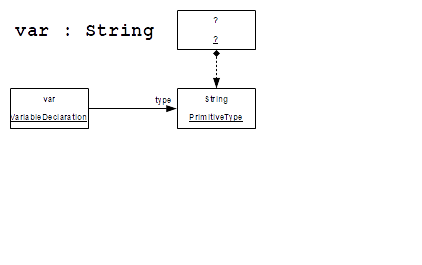
\includegraphics[width=4.5in]{OCL2TypeReference.png}
	\end{center}
	\vspace{-110pt}
	\caption{OCL 2 Type Reference}
	\label{fig:OCL2TypeReference}
\end{figure}

\begin{verbatim}
    var : Set(String)
\end{verbatim}

The \verb$VariableDeclaration::type$ must now point to some type that is constructed or re-used on behalf of the reference. The OCL~2 specification provides no clues, although in response to the issue that I raised, \verb$ExpressionInOCL::generatedType$ was added in OCL~2.2 without any indication of how it solves the problem or ensures uniqueness.

The \verb$MetamodelManager$ brings order to this anarchy by supervising the model elements that may be built-in to the tooling, form part of a library, form part of a user metamodel or which may be constructed on demand to satisfy the need for a unique definition of a synthesized type. Figure~\ref{fig:OCL3TypeDescriptor} shows a \verb$MetamodelManager$ with transitive containment via omitted packages and models to the built-in library \verb$PrimitiveType$ instance and the synthesized \verb$SetType$ instance.

\begin{figure}
	\begin{center}
		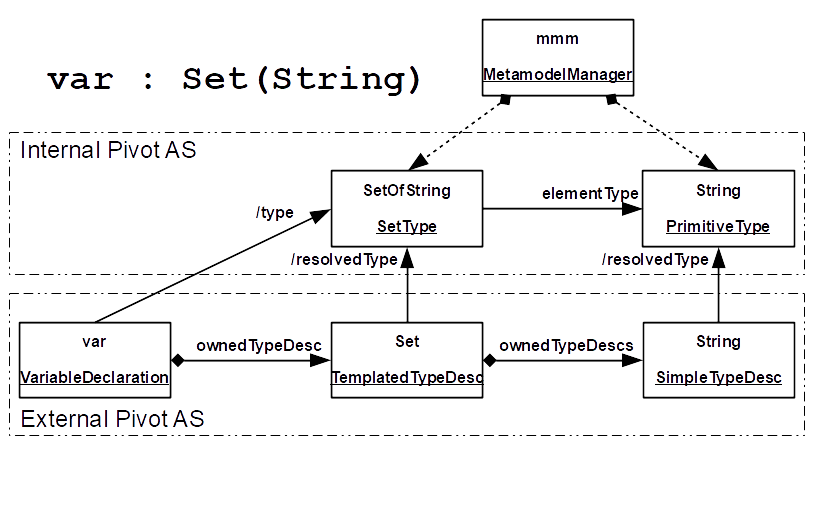
\includegraphics[width=4.5in]{OCL3TypeDescriptor.png}
	\end{center}
	\vspace{-40pt}
	\caption{Possible OCL 3 Type Descriptor}
	\label{fig:OCL3TypeDescriptor}
\end{figure}

In order to isolate the parser from the complexities of locating unique definitions, the \verb$VariableDeclaration::type$ property is changed to a derived property that is part of the internal perspective. The \verb$VariableDeclaration::ownedTypeDesc$ external perspective property is populated by the parser with a description of the referenced type. This description is locally contained by the referencing \verb$VariableDeclaration$ and so may be as complicated as necessary. In the example, the \verb$Set$ is parsed as a \verb$TemplatedTypeDesc$ parameterized by a \verb$Set$ name and \verb$String$ template parameter. The template parameter is parsed as a \verb$SimpleTypeDesc$ parameterized by a \verb$String$ name. Each type descriptor has a lazily resolved \verb$TypeDesc::resolvedType$ derived property as its internal perspective. 




%In this case an adjustment to the AS to accommodate direct parsing solves a significant XMI serialization issue for free. No change to the textual concrete syntax is necessary.

%An example of the benefits of revisiting the AS can be seen by considering the problem of referencing a type as in:

%It seems obvious that the AS should have a \verb$VariableDecaration::type$ property so that the instance of \verb$Variable$ has a \verb$type$ reference to the type whose name is \verb$String$. 

%This is shown in Figure~\ref{fig:OCL2TypeReference} and is exactly what the OCL~2 specification defines. The Figure is a UML instance diagram with additional decorations to show compositions. The containment of the PrimitiveType is unclear.

%The design is poor since its support for synthesized template types is troubled.

%\begin{verbatim}
%var : Set(String)
%\end{verbatim}

%Somehow the a definition of \verb$Set(String)$ must be located to terminate the \verb$VariableDeclaration::type$ reference. Where is that definition? Presumably it must be unique, so there is an additional problem in ensuring uniqueness if \verb$Set(String)$ is referenced from multiple XMI serializations. The OCL specification provides no answers, although in response to the issue that I raised, \verb$ExpressionInOCL::generatedType$ was added in OCL~2.2 without any indication of how it solves the problem or ensures uniqueness.

%The problem is that in the textual concrete syntax we have type descriptions such as \verb$Set(String)$ that are repeated for every distinct usage. \verb$String$ too is a six letter type description that converts to a primitive type.

%To facilitate parsing we need a model that supports type descriptions; the non-normative CS classes do exactly this for OCL~2. But to facilitate OCL execution we would like a more streamlined AS representation that references the described type. Currently the conflict is resolved by incurring an awkward CS2AS conversion phase.

%If we accept that a little bloat of the OCL AS is acceptable, we can have a \verb$VariableDeclaration::ownedTypeDesc$ composed property and a \verb$VariableDeclaration::type$ derived transient property. The composed \verb$VariableDeclaration::ownedTypeDesc$ property owns an object tree that describes the referenced type and is constructed directly by the parser similar to the OCL~2 CS. The derived \verb$VariableDeclaration::type$ property references the resolved type just as the 




%many asupervises the Pivot metamodel representation normalized by the loader transformation from the user's preferred metamodel representation. 





%Fig~\ref{fig:OCL3Architecture} shows a simpler and more regular architecture that might be adopted for OCL~3. 

%\subsubsection{Summary}

%The \verb$MetamodelManager$ supervises the Pivot metamodel representation normalized by the loader transformation from the user's preferred metamodel representation. 

%The distinct CST and ASG are replaced by a single dual-perspective Pivot AS.

%The external aspects comprise element descriptors populated by the parser. The external aspects can be interchanged using XMI. 

%The internal aspects comprise the uniquely resolved elements for each descriptor. The resolutions use derived transient properties whose body invokes a \verb$MetamodelManager$ query using the reserved variable \verb$mmm$.

%The transient internal uniquely resolved aspects are determined by derived properties that use the \verb$MetamodelManager$ to resolve element descriptions to the normalized elements loaded from user metamodels. 

%The \verb$ModelManager$ performs model loading and value normalization on behalf of the evaluator.

%Revision of the grammar and AS to avoid ambiguities avoids the need for non-standard parser disambiguation.

%Replacing the distinct CST and ASG by external and internal aspects of a single Pivot AS avoids the need for non-standard parser resolution and facilitates interchange with XMI.
%But how? Important classes such as \verb$Package$, \verb$Class$, \verb$Property$, \verb$Operation$, \verb$Constraint$ are missing. The specification just loosely suggests that the equivalents from your favourite metamodeling language can be used, specifically assuring that the EssentialOCL is compatible with EMOF even though EMOF (and Ecore) has no \verb$Constraint$ class at all. Some Ecore tools struggle to extend Ecore with a missing \verb$EConstraint$. Eclipse OCL struggles with magic overloads of \verb$EAnnotation$.



\subsubsection{XMI}

The OCL~2 specification calls for model interchange between tools using XMI but leaves many awkward challenges such as references to unnavigable opposites and references to additional operations and containment of synthesized types unresolved.

Since OCL~2 has survived without XMI for 20 years, we could just eliminate this specification point, but given a sensibly designed metamodel XMI should be easy.

The problem with XMI for OCL~2 is the need to serialize references to awkward definitions. With the two perspective AS suggested above, the external perspective comprises descriptors for the definitions avoiding the difficulties. After an XMI load, the descriptors can be resolved in a very similar fashion to the lazy resolution after parsing.

\subsubsection{Open classes}

The ability to add attributes and operations to classes is difficult to support when their AS representation is to be just like similar attributes and operations defined in the model. This problem led Eclipse OCL to prototype a solution whereby a complete-Class was an overlay of same-named partial-Classes enabling the additional definitions to be overlaid on the primary definition and serialized in a similar fashion. This gives a powerful but non-trivial transitive Package merge capability for same-URI packages. Is it really necessary?

Many modeling capabilities such as Acceleo~\cite{Eclipse-Acceleo}, ATL~\cite{Eclipse-ATL} and QVTo~\cite{Eclipse-QVTo} support additional features as helper operations and helper attributes. They are clearly useful and an important aid to modularization of non-trivial OCL constraints. The deliberate avoidance of such helpers by the UML~2.5~\cite{UML-2.5} specification leads to some long unreadable repetitive OCL expressions. This clearly demonstrates their utility.

However we only need helper features and so a reversion to the OCL~1.x pseudo-features would suffice. With an AS serialization that serializes references as descriptors rather than resolved references, the problem of where the referenced definition exists is no longer a problem.

\subsubsection{Grammar Rationalization}

Where the grammar is bad there are only two choices.

\begin{itemize}
	\item Require skilled implementers to provide trickery to workaround the bad grammar
	\item Change the grammar to something sensible
\end{itemize}

The former approach is incompatible with our goal of a simple re-usable grammar, so a textual syntax change is unavoidable.

The major syntax problem arises through the introduction of prefix declarations for a long form iteration call such as

\begin{verbatim}
    aCollection->forAll(e1, e2 | ...)
\end{verbatim}

This requires undue lookahead through the iterators to find the \verb$|$ that distinguishes the iterator call syntax from the similar operation call syntax

\begin{verbatim}
    aCollection->myForAll(e1, e2)
\end{verbatim}

Most of the OCL syntax is freeform which is friendly but can be challenging. Where the freeform is too hard, additional keywords such as \verb$let$ or \verb$endif$ ensure that the parser knows exactly what is happening.

If we introduce the \verb$var$ keyword for variable declarations, we can rewrite the iteration call as

\begin{verbatim}
    aCollection->forAll(var e1; var e2; ...)
\end{verbatim}

in which each \verb$var ... ;$ clause is a prefix to the subsequent OCL expression. In this case the variable type can be inferred.

This syntax can be re-used to eliminate the let syntax by rewriting:

\begin{verbatim}
    let x = ... in
    let y = ... in 
    ...
\end{verbatim}

as

\begin{verbatim}
    var x := ...;
    var y := ...; 
    ...
\end{verbatim}

This change also solves the dangling-in parsing challenge that arises when let expressions are nested carelessly. This change should also unblock my failed prototype of an OCL extension to support QVTr-like patterns that in one trivial example avoids the clumsy need for an \verb$oclIsKindOf(CastX)$ immediately followed by a matching \verb$oclAsType(CastX)$.

\begin{verbatim}
    if (var castX : CastX := x)     -- x.oclIsKindOf(CastX)
    then castX.doSomething()        -- x.oclAsType(CastX).doSomething()
    else null
    endif
\end{verbatim}

\section{Conclusion}\label{Conclusion}

We have shown how the well-intentioned upgrade of the simple but useful OCL~1 specification went astray as part of the UML~2 activities. We have identified that draft work-in-progress was accidentally adopted as the OMG OCL~2 specification.

We have drawn on personal experiences to explain why OCL tool implementers treated the OCL~2 specification with unwarranted reverence and so struggled to implement it as faithfully as possible.

It is a pity that it has taken so long to recognise the OCL~2 specification for the disaster that it is.

We make proposals for an OCL~3 that can almost be seen as going back to OCL~1 and then moving forwards again to avoid the mistakes of OCL~2.

\backmatter

\bibliographystyle{alphaurl}
\bibliography{OCLReflections}

\abouttheauthors

%\begin{acknowledgments}
%Many thanks to Horacio Hoyos Rodriguez for the graphical perspective and Epsilon prototype and to all Dimitris Kolovos' team for insightful discussions.
%\end{acknowledgments}

\end{document}


